\documentclass[oneside,10pt]{book}

\usepackage{cdtBook}
\usepackage{usecases}

\title{Clinica}
\subtitle{Clinica de Homeopatia}
\author{Barrios Alvarado Daniel Alejandro\\ Cabello Acosta Gerardo Aramis\\ Cuellar Sanchez Ricardo\\ Maldonado Ledo Diana Guadalupe\\}
        
%\organization{Escuela Superior de C�mputo, IPN}


%%%%%%%%%%%%%%%%%%%%%%%%%%%%%%%%%%%%%%%%%%%%%%%%%%%%%%%%%%%%%%%%
\begin{document}

\maketitle
\thispagestyle{empty}

\frontmatter
\tableofcontents

\mainmatter

%=========================================================
\chapter{Introducci�n}

\cfinput{introduccion}

%=========================================================
\chapter{An�lisis del problema}

\cfinput{problematica}

%=========================================================
\chapter{Propuesta de soluci�n}

\cfinput{propuesta}



%=========================================================
\chapter{Modelo de Negocios}

\cfinput{brGlosario}
\cfinput{brProceso}
\cfinput{brModelo}
\cfinput{brReglas}

%=========================================================
\chapter{Modelo del despliegue del sistema}

%=========================================================
\chapter{Modelo de comportamiento}
	
	%\begin{figure}[htbp!]
	%	\centering
	%		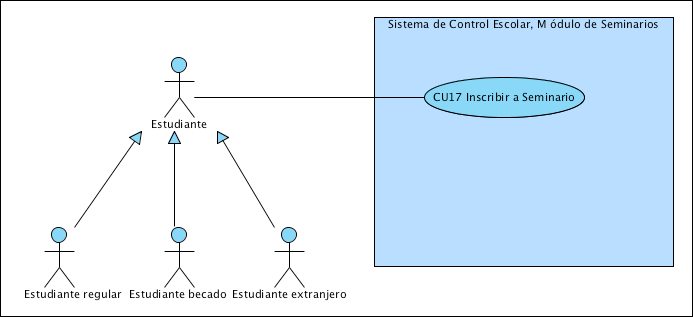
\includegraphics[width=0.8\textwidth]{images/CasosDeUso}
	%	\caption{Diagrama de Casos de Uso del sistema.}
	%\end{figure}
\cfinput{modeloComportamiento}

%\cfinput{cu17/cu}
%\cfinput{cu1/cu}
%\cfinput{cu2/cu}
%\cfinput{cu3/cu}
%\cfinput{cu4/cu}
%\cfinput{cu5/cu}

%%=========================================================
\chapter{Modelo de la Interacci�n}

\cfinput{Pantallas/navegacion}

\cfinput{Pantallas/IU23}
%\cfinput{Pantallas/IU1}
%\cfinput{Pantallas/IU2}
%\cfinput{Pantallas/IU3}
%\cfinput{Pantallas/IU4}
%\cfinput{Pantallas/IU5}
%\cfinput{Pantallas/IU6}
%\cfinput{Pantallas/IU7}

	
\end{document}